\subsection{妇女事业发展的推进}
\begin{frame}{中国高度重视并积极推进妇女事业发展}
    \begin{block}{}
        \begin{itemize}
            \item 促进妇女全面发展和男女平等是中国特色社会主义的重要组成部分。
            \item “坚持男女平等基本国策,保障妇女儿童合法权益”写入党的十八大、十九大报告,成为党治国理政的重要理念和内容。
            \item 建立完善人大立法保障妇女权益的工作机制。
            \item 建立完善政协协商推动妇女事业发展的工作机制。
            \item 建立健全政府贯彻落实男女平等基本国策的工作机制。
            \item 建立健全妇联组织作为党和政府联系妇女群众桥梁纽带的工作机制。
        \end{itemize}
    \end{block}
\end{frame}

\begin{frame}{中国高度重视并积极推进妇女事业发展}
    \begin{center}
        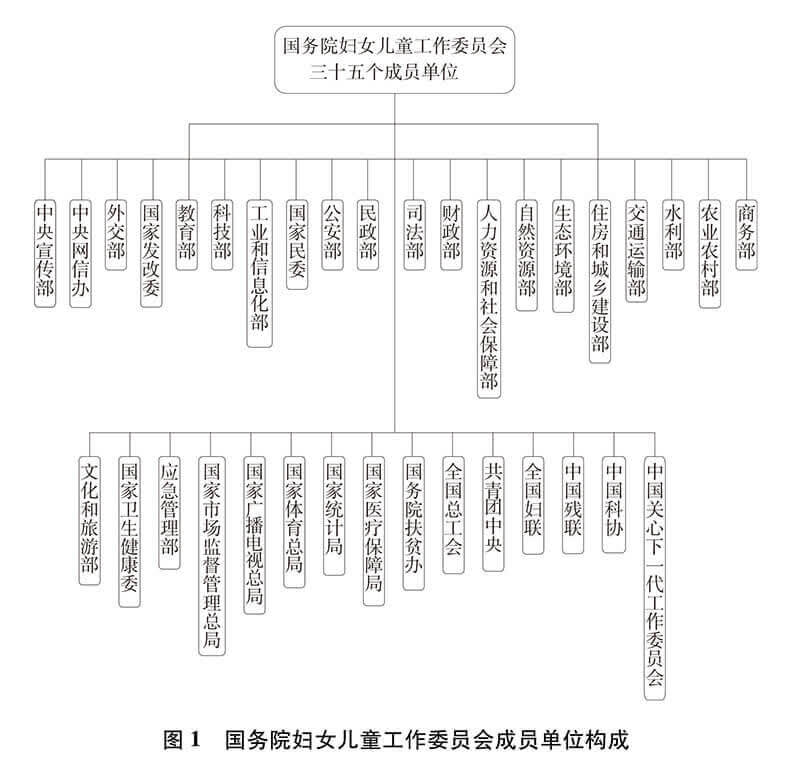
\includegraphics[width=.55\textwidth]{../docs/img/2-1.jpg}
    \end{center}
\end{frame}

\begin{frame}{中国高度重视并积极推进妇女事业发展}
    \begin{center}
        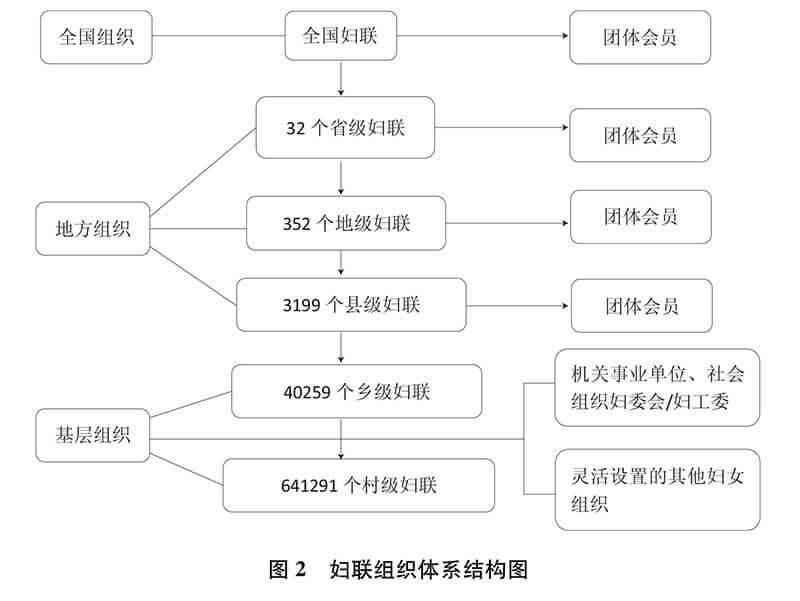
\includegraphics[width=.7\textwidth]{../docs/img/2-2.jpg}
    \end{center}
\end{frame}



\subsection{妇女权益保障体系的完善}
\begin{frame}{保障妇女权益的法治体系不断完善}
    \begin{block}{}
        \begin{itemize}
            \item 妇女权益是基本人权。中国把保障妇女权益纳入法律法规,上升为国家意志,内化为社会行为规范。
            \item 保障妇女权益的法治宣传深入普及。将保障妇女权益的法律知识、法治精神、法治文化纳入全民普法规划。
        \end{itemize}
    \end{block}
    \begin{center}
        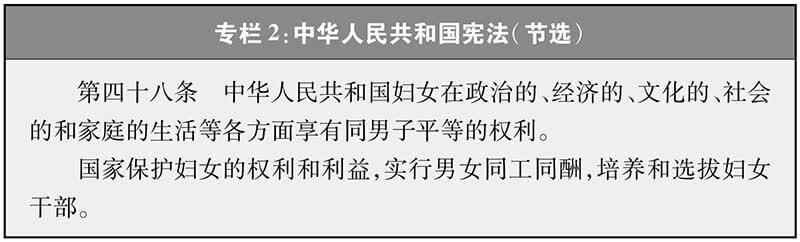
\includegraphics[width=\textwidth]{../docs/img/2-3.jpg}
    \end{center}
\end{frame}



\subsection{妇女在经济社会发展的作用}
\begin{frame}{妇女在经济社会发展中的半边天作用日益彰显}
    \begin{block}{}
        \begin{itemize}
            \item 妇女在脱贫攻坚中充分参与、广泛受益。中国高度重视妇女扶贫脱贫。
            \item 保障平等土地权益调动农村妇女生产积极性。
            \item 全社会就业人员中女性占比超过四成。
        \end{itemize}
    \end{block}
    \begin{center}
        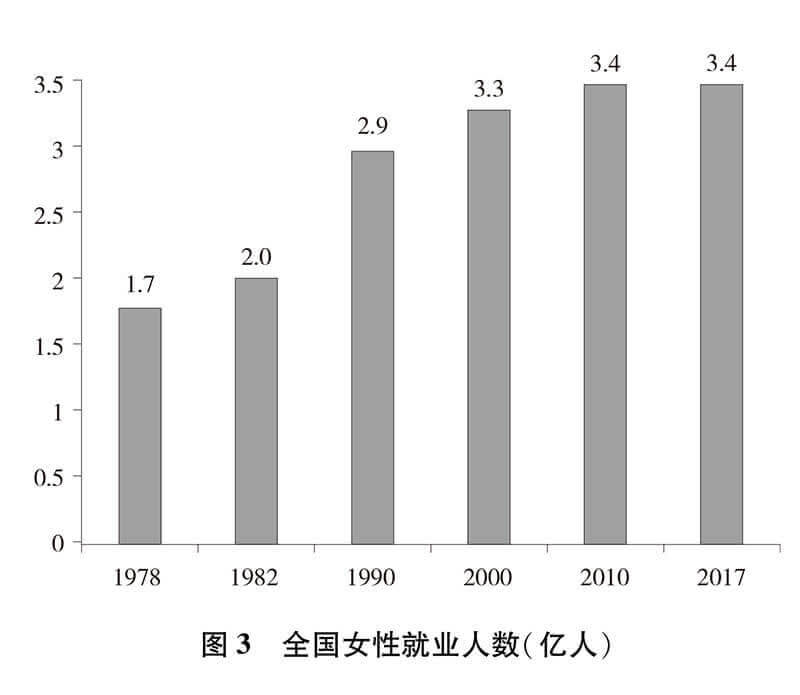
\includegraphics[width=.45\textwidth]{../docs/img/2-4.jpg}
    \end{center}
\end{frame}



\subsection{妇女政治地位的显著提高}
\begin{frame}{妇女政治地位显著提高}
    \begin{block}{}
        \begin{itemize}
            \item 中国共产党作为执政党,一贯重视培养选拔女干部、发展女党员。人大代表和政协委员中女性比例逐步提升。
        \end{itemize}
    \end{block}
\end{frame}



\subsection{妇女受教育水平的显著提升}
\begin{frame}{妇女受教育水平显著提升}
    \begin{center}
        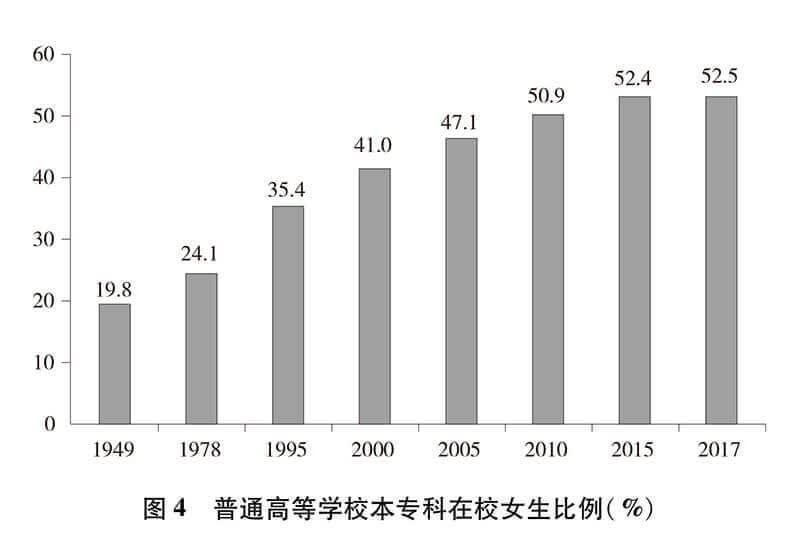
\includegraphics[width=.8\textwidth]{../docs/img/2-5.jpg}
    \end{center}
\end{frame}



\subsection{妇女健康状况的极大改善}
\begin{frame}{妇女健康状况极大改善}
    \begin{center}
        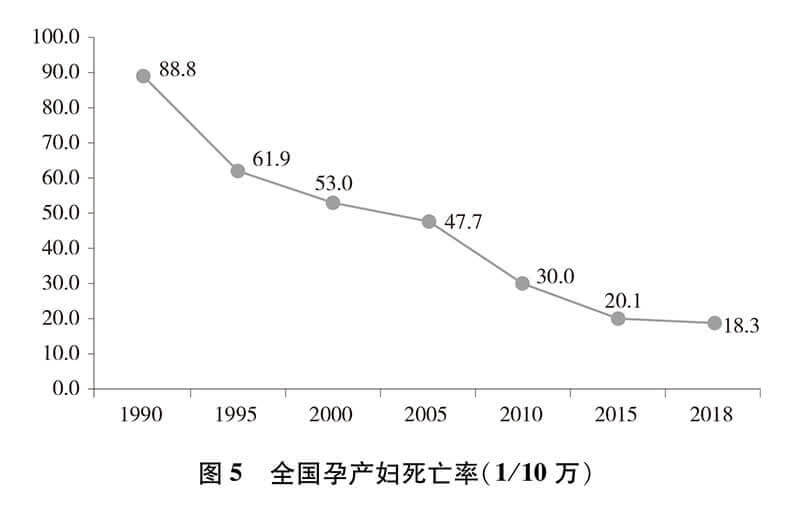
\includegraphics[width=.8\textwidth]{../docs/img/2-6.jpg}
    \end{center}
\end{frame}



\subsection{妇女社会保障水平的提高}
\begin{frame}{妇女社会保障水平不断提高}
    \begin{center}
        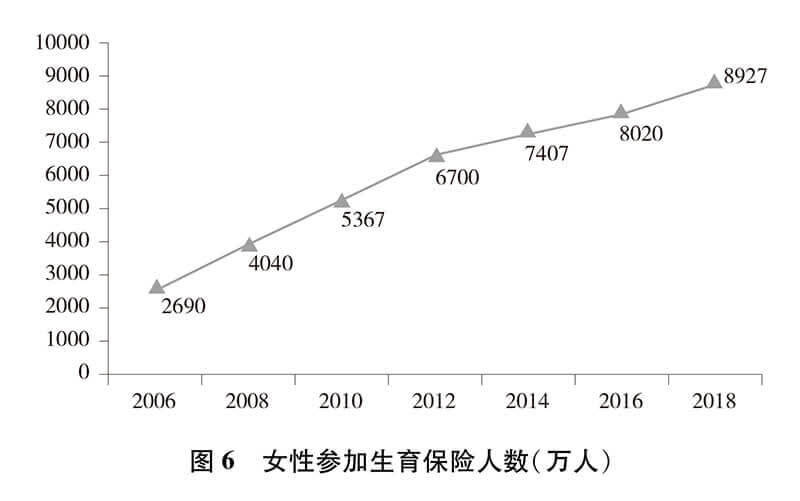
\includegraphics[width=.8\textwidth]{../docs/img/2-7.jpg}
    \end{center}
\end{frame}



\subsection{妇女在家庭文明建设的作用}
\begin{frame}{妇女在家庭文明建设中发挥独特作用}
    \begin{center}
        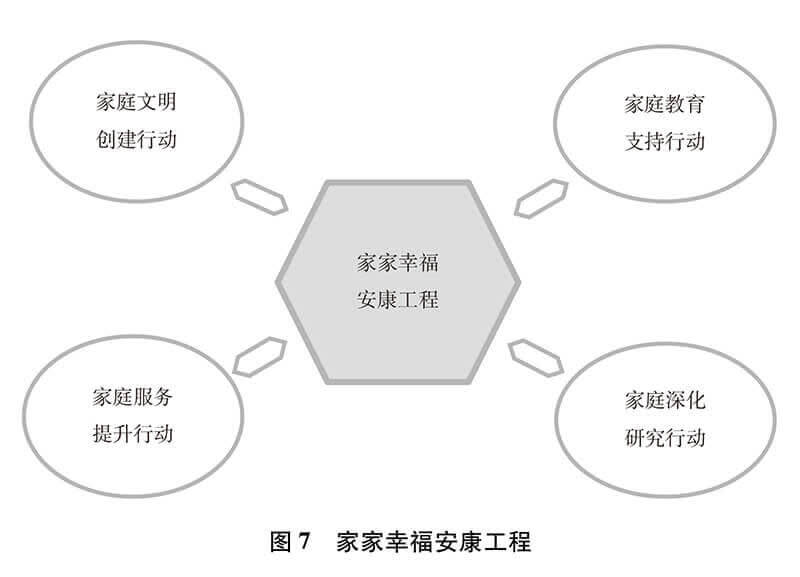
\includegraphics[width=.7\textwidth]{../docs/img/2-8.jpg}
    \end{center}
\end{frame}
